\section{机器学习概念}

\begin{definition}[机器学习]
    机器学习能使计算机能够在没有明确编程的情况下学习。

    一个计算机程序从经验 $E$ 中学习任务 $T$，并用性能 $P$ 来衡量表现。
\end{definition}

\begin{definition}[特征编码]
    主要目的就是为了将各种类型的非数值数据，比如文本、分类变量（如颜色、性别）等，转换为机器学习模型可以理解和处理的数值格式。
\end{definition}

\subsection{编码方法}

\begin{definition}[编码方法]
    为了让模型能够处理不同类型的变量，我们通常需要将它们转换为数值格式。这个过程就是特征编码。根据变量类型的不同，我们可以选择不同的编码方法。
\end{definition}

\begin{example}[无序类别变量的独热编码]
    对于没有内在顺序关系的变量，如颜色或性别，我们使用\textbf{独热编码} (\texttt{One-Hot Encoding})。该方法为每个类别创建一个新的二进制特征列。
    例如：
    \begin{center}
        \begin{itemize}
            \item 红色 $\rightarrow [1, 0, 0]$ \quad \quad 蓝色 $\rightarrow [0, 1, 0]$ \quad \quad 绿色 $\rightarrow [0, 0, 1]$
        \end{itemize}
    \end{center}
\end{example}

\begin{example}[有序类别变量的标签编码]
    对于具有明确顺序或等级关系的变量，如评级或教育程度，我们使用\textbf{标签编码} (\texttt{Label Encoding})。该方法将每个类别映射为一个唯一的整数。
    例如：
    \begin{center}
        \begin{itemize}
            \item 差 $\rightarrow 0$ \quad \quad 中 $\rightarrow 1$ \quad \quad 优 $\rightarrow 2$
        \end{itemize}
    \end{center}
\end{example}

\begin{example}[数值变量的标准化与归一化]
    对于数值变量，我们通常需要进行尺度调整，以提升模型性能。
    \begin{itemize}
        \item \textbf{标准化}：将数据转换为均值为 $0$ ，标准差为 $1$ 的分布，公式为：
              \begin{align*}
                  x' = (x - \mu) / \sigma
              \end{align*}
        \item \textbf{归一化}：将数据缩放到固定范围，如 $[0, 1]$，公式为：
              \begin{align*}
                  x' = (x - x_{\min}) / (x_{\max} - x_{\min})
              \end{align*}
    \end{itemize}
\end{example}

\begin{example}[文本数据的编码]
    对于文本数据，常用的编码方法有：
    \begin{enumerate}
        \item \textbf{词袋模型}：将文档表示为词频向量，忽略词语顺序。
        \item \textbf{TF-IDF}：在词频基础上，考虑词语在整个语料库中的重要性。
        \item \textbf{词嵌入}：将词语映射到低维向量，捕捉词语间的语义和语法关系。
    \end{enumerate}
\end{example}

\section{机器学习类型}

\begin{definition}[监督学习]
    监督学习是一种机器学习方法，其中算法从标记的训练数据中学习，以预测新数据的输出。训练数据包含输入特征和对应的正确输出（标签）。

    监督学习主要分为两类任务：
    \begin{enumerate}
        \item \textbf{分类}：预测离散的类别标签
              \begin{itemize}
                  \item 二分类：垃圾邮件检测（垃圾/非垃圾）
                  \item 多分类：图像识别（猫/狗/鸟）
              \end{itemize}
        \item \textbf{回归}：预测连续的数值
              \begin{itemize}
                  \item 房价预测、股票价格预测
              \end{itemize}
    \end{enumerate}
\end{definition}

\begin{definition}[样本]
    样本：$s_i=\left(\mathbf{x}_i, y_i\right)$。样本是特征向量和标签的组合。在数据集中，每个样本代表一个独立的观测或实例。
\end{definition}

训练过程大致如下：

给定训练数据：$\left\{\left(\mathbf{x}^1, y^1\right),\left(\mathbf{x}^2, y^2\right), \ldots,\left(\mathbf{x}^N, y^N\right)\right\}$
训练的过程是 3 个步骤：
\begin{enumerate}
    \item 建立模型：建立带末知参数 $\theta$ 的函数 $f_\theta(\mathbf{x})$ ，其中 $\theta$ 代表模型里全部待学习的参数。
    \item 定义损失：构造损失函数 $L(\theta)$ ，它以参数 $\theta$ 为输入，衡量这组参数在训练集上的好坏程度。
    \item 优化求解：求解 $\theta^*=\arg \min _\theta L(\theta)$ 得到最优参数 $\theta^*$ 。
\end{enumerate}

则函数 $f_{\theta^*}(\mathbf{x})$ 就是所求模型

\begin{definition}[无监督学习]
    无监督学习是从没有标签的数据中发现隐藏模式和结构的机器学习方法。算法需要在没有正确答案指导的情况下，自主发现数据中的规律。
\end{definition}

\begin{example}[无监督学习任务类型]
    无监督学习的主要任务包括：
    \begin{enumerate}
        \item \textbf{聚类}：将相似的数据点分组
              \begin{itemize}
                  \item K-means 聚类、层次聚类
              \end{itemize}
        \item \textbf{降维}：减少数据的特征维度
              \begin{itemize}
                  \item 主成分分析（PCA）、t-SNE
              \end{itemize}
        \item \textbf{关联规则挖掘}：发现数据项之间的关联关系
              \begin{itemize}
                  \item 购物篮分析、推荐系统
              \end{itemize}
    \end{enumerate}
\end{example}

\begin{definition}[强化学习]
    强化学习是一种通过与环境交互来学习最优行为策略的机器学习方法。智能体通过执行动作、观察环境状态变化和获得奖励来学习。
\end{definition}

\section{机器学习三要素}

\subsection{模型}

\begin{definition}[决策函数模型]
    记 $X$ 是任一特征向量，$Y$ 是任一标签。决策函数模型：
    $$Y=f(\mathbf{X})$$
    例如，线性回归模型就是一个决策函数模型，它通过线性组合特征向量的元素来预测标签。
    可以理解为，对于分类问题，模型学习一个函数 $f(x)$ 。当 $f(x)$ 的值大于某个阈值（通常是 0 ）时，就判为正类；小于阈值时，就判为负类：
    $$
        y=\operatorname{sign}(f(x))
    $$
    其中 $y$ 是预测的类别（例如 +1 或 -1 ），$x$ 是输入的特征向量。
\end{definition}

\begin{definition}[概率模型]
    概率模型（给定特征向量 $X$ 时，标签 $Y$ 的概率分布）：
    $$\quad P(Y \mid \mathbf{X})$$
    例如，逻辑回归模型就是一个概率模型，它通过特征向量来预测标签为某个特定值的概率。输出的是一个概率分布。

    模型学习的是条件概率 $P(y \mid x)$ 。预测时，我们会选择概率最大的那个类别作为最终结果：
    $$
        \hat{y}=\arg \max _y P(y \mid x)
    $$
    其中 $\hat{y}$ 是预测的类别。
\end{definition}

\begin{definition}[假设空间]
    所有可能的决策函数或者条件概率分布的集合决策函数集合：包含了所有可能的决策函数，其中 $\theta$ 是模型的参数。
    $$\mathcal{H}=\left\{f \mid Y=f(\mathbf{X} ; \theta), \theta \in \mathbb{R}^n\right\}$$
    条件概率的集合：包含了所有可能的条件概率分布，其中 $\theta$ 是模型的参数。
    $$\mathcal{H}=\left\{P \mid P(Y \mid \mathbf{X} ; \theta), \theta \in \mathbb{R}^n\right\}$$
    学习过程的目标是从假设空间中选择一个最佳模型。
\end{definition}

\subsection{策略}

\begin{definition}[策略]
    根据评价准则，从假设空间中选择最优模型的方法。
\end{definition}

\begin{definition}[损失函数]
    损失函数是衡量模型预测值与真实值之间差异的函数，它定义了模型在单个样本上的误差。损失函数的目的是量化模型的预测性能，以便在训练过程中通过优化算法最小化这个误差。不同的损失函数适用于不同的任务和模型。

    $0-1$ 损失函数：
    $$
        L(Y, f(\mathbf{X}))=\mathbb{I}(f(\mathbf{X}) \neq Y)= \begin{cases}1, & f(\mathbf{X}) \neq Y \\ 0, & f(\mathbf{X})=Y\end{cases}
    $$
    平方损失函数：
    $$
        L(Y, f(\mathbf{X}))=(Y-f(\mathbf{X}))^2
    $$
    绝对损失函数：
    $$
        L(Y, f(\mathbf{X}))=|Y-f(\mathbf{X})|
    $$
    对数损失函数：
    $$L(Y, P(Y \mid \mathbf{X}))=-\log P(Y \mid \mathbf{X})$$
\end{definition}

\begin{definition}[期望风险]
    模型在所有未知数据上的平均损失，代表模型的真实泛化能力。
    $$
        R_{\text{exp}}(f) = \int_{X \times Y} L(y, f(x)) P(x, y) \,dx\,dy
    $$
    $P(x,y)$ 可以视作是全部试题，这是做不完的，所以监督学习是一个病态问题。
\end{definition}

\begin{definition}[经验风险]
    模型在给定训练集上的平均损失，是对期望风险的近似估计。
    $$
        R_{\text{emp}}(f) = \frac{1}{N} \sum_{i=1}^{N} L(y_i, f(x_i))
    $$
    相当于手上的练习册，我们能做的就只是降低经验风险。
    \begin{itemize}
        \item 模型的目标不仅仅是对训练数据拟合得好（即训练误差小）
        \item 更重要的是在未见过的新数据上也能表现良好（即泛化误差小）
    \end{itemize}

\end{definition}



\section{模型评估与选择}

\begin{definition}[训练集、验证集和测试集]
    为了正确评估模型性能，通常将数据集划分为三部分：
    \begin{itemize}
        \item \textbf{训练集}：用于训练模型参数
        \item \textbf{验证集}：用于调整超参数和模型选择
        \item \textbf{测试集}：用于最终评估模型的泛化性能
    \end{itemize}
    典型的划分比例为 $60\%:20\%:20\%$ 或 $70\%:15\%:15\%$。
\end{definition}

\begin{definition}[交叉验证]
    交叉验证是一种模型评估技术，通过多次划分数据集来获得更可靠的性能估计。最常用的是 $k$ 折交叉验证：
    \begin{enumerate}
        \item 将数据集随机划分为 $k$ 个大小相等的子集
        \item 每次使用 $k-1$ 个子集作为训练集，剩余 $1$ 个子集作为验证集
        \item 重复 $k$ 次，每次选择不同的验证集
        \item 最终性能为 $k$ 次验证结果的平均值
    \end{enumerate}
\end{definition}

\section{常见算法}

\begin{definition}[线性回归]
    线性回归是最基础的回归算法，假设目标变量与特征变量之间存在线性关系：

    $$y = \beta_0 + \beta_1 x_1 + \beta_2 x_2 + \cdots + \beta_n x_n + \epsilon$$

    其中 $\beta_i$ 是回归系数，$\epsilon$ 是误差项。
\end{definition}

\begin{definition}[逻辑回归]
    逻辑回归用于二分类问题，使用 Sigmoid 函数将线性组合映射到 $[0,1]$ 区间：

    $$P(y=1|x) = \frac{1}{1 + e^{-(\beta_0 + \beta_1 x_1 + \cdots + \beta_n x_n)}}$$
\end{definition}

\begin{definition}[决策树]
    决策树是一种基于树结构的分类和回归方法，通过一系列判断条件将数据递归地划分为更纯净的子集。
    \begin{itemize}
        \item \textbf{信息增益}：衡量特征对分类纯度提升的贡献
        \item \textbf{基尼不纯度}：衡量节点中类别混合程度的指标
        \item \textbf{剪枝}：防止过拟合的技术
    \end{itemize}
\end{definition}

\begin{definition}[支持向量机（SVM）]
    SVM 通过寻找最优超平面来分离不同类别的数据点，最大化类别间的间隔（margin）。
    \begin{itemize}
        \item \textbf{支持向量}：距离超平面最近的数据点
        \item \textbf{核技巧}：将数据映射到高维空间以处理非线性问题
        \item 常用核函数：线性核、多项式核、RBF核
    \end{itemize}
\end{definition}

\section{模型性能指标}

\begin{definition}[分类问题的评估指标]
    对于分类问题，常用的评估指标包括：
    \begin{itemize}
        \item \textbf{准确率}：$\text{Accuracy} = \frac{TP + TN}{TP + TN + FP + FN}$
        \item \textbf{精确率}：$\text{Precision} = \frac{TP}{TP + FP}$
        \item \textbf{召回率}：$\text{Recall} = \frac{TP}{TP + FN}$
        \item \textbf{F1分数}：$\text{F1} = 2 \times \frac{\text{Precision} \times \text{Recall}}{\text{Precision} + \text{Recall}}$
    \end{itemize}
    其中，TP（真正例）、TN（真负例）、FP（假正例）、FN（假负例）。
\end{definition}

\begin{definition}[回归问题的评估指标]
    对于回归问题，常用的评估指标包括：
    \begin{itemize}
        \item \textbf{均方误差}：$\text{MSE} = \frac{1}{n}\sum_{i=1}^{n}(y_i - \hat{y}_i)^2$
        \item \textbf{均方根误差}：$\text{RMSE} = \sqrt{\text{MSE}}$
        \item \textbf{平均绝对误差}：$\text{MAE} = \frac{1}{n}\sum_{i=1}^{n}|y_i - \hat{y}_i|$
        \item \textbf{决定系数}：$R^2 = 1 - \frac{\sum_{i=1}^{n}(y_i - \hat{y}_i)^2}{\sum_{i=1}^{n}(y_i - \bar{y})^2}$
    \end{itemize}
    其中，$y_i$ 是真实值，$\hat{y}_i$ 是预测值，$\bar{y}$ 是真实值的均值。
\end{definition}

\section{过拟合与欠拟合}

\begin{definition}[过拟合]
    过拟合是指模型在训练数据上表现很好，但在新数据上表现较差的现象。模型过度学习了训练数据中的噪声和细节，导致泛化能力下降。
\end{definition}

\begin{definition}[欠拟合]
    欠拟合是指模型过于简单，无法捕捉数据中的基本模式，在训练数据和测试数据上都表现较差。
\end{definition}

\begin{figure} [H]
    \centering
    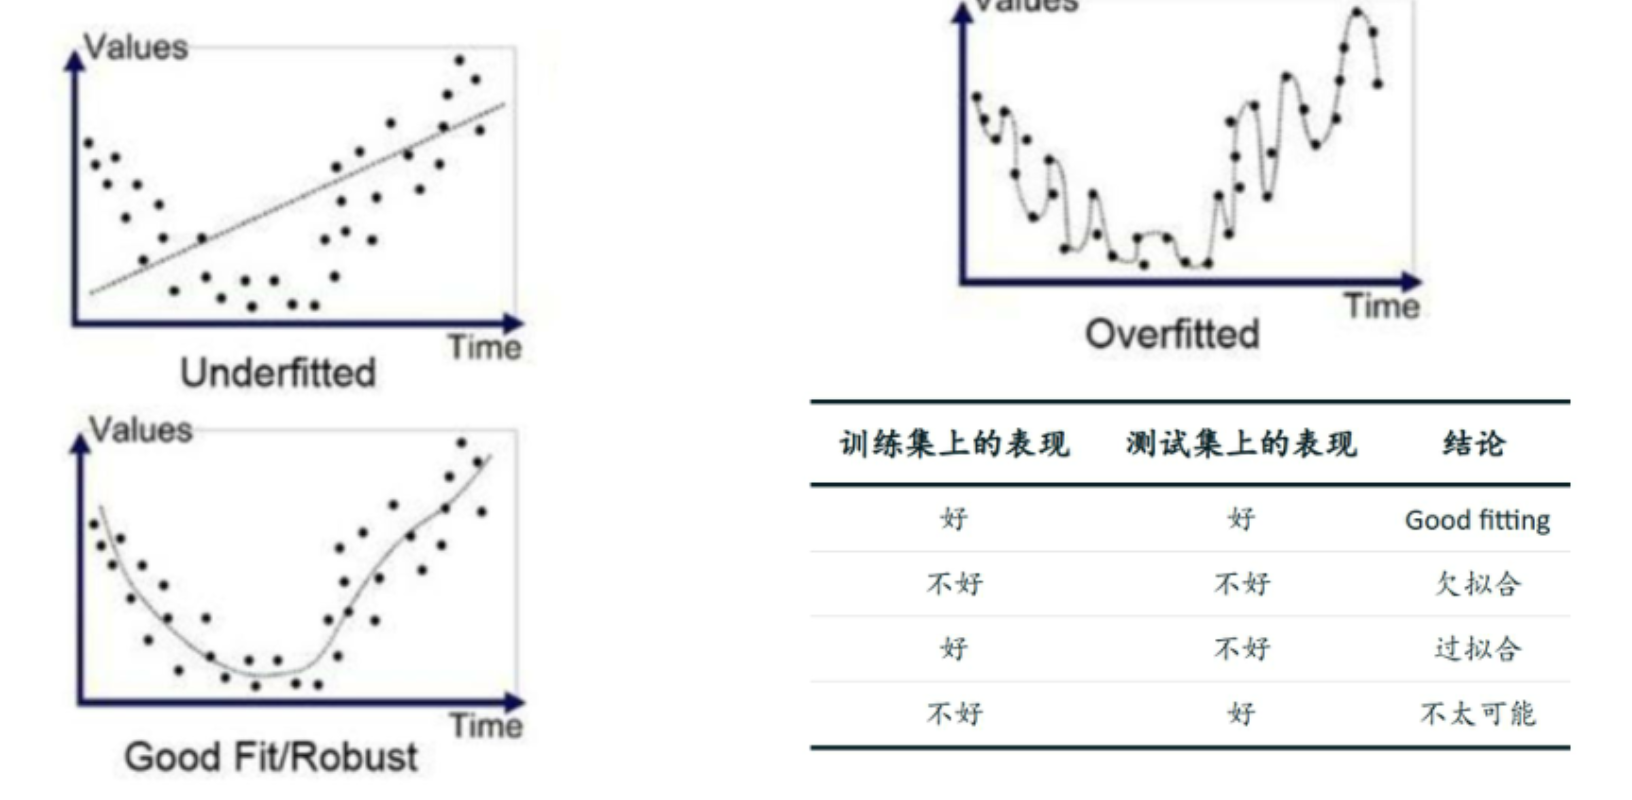
\includegraphics[width=0.65\textwidth]{chapters/机器学习/images/机器学习概念/img-20250926133200.png}
\end{figure}

\begin{definition}[模型复杂度]
    越复杂的模型对数据的描述能力越强，但过度学习的风险也很大。模型复杂度较低容易欠拟合，模型复杂度较高容易过拟合。
\end{definition}



\begin{example}[防止过拟合的方法]
    常用的防止过拟合的技术包括：
    \begin{enumerate}
        \item \textbf{正则化}：在损失函数中添加惩罚项
              \begin{itemize}
                  \item L1正则化（Lasso）：$\lambda \sum_{i=1}^{n}|\beta_i|$
                  \item L2正则化（Ridge）：$\lambda \sum_{i=1}^{n}\beta_i^2$
              \end{itemize}
        \item \textbf{早停}：在验证误差开始上升时停止训练
        \item \textbf{Dropout}：随机丢弃部分神经元（深度学习中）
        \item \textbf{数据增强}：增加训练数据的多样性
        \item \textbf{集成方法}：结合多个模型的预测结果
    \end{enumerate}
\end{example}

\section{集成学习}

\begin{definition}[集成学习]
    集成学习通过组合多个学习器的预测结果来提高整体性能。基本思想是"三个臭皮匠，顶个诸葛亮"。
\end{definition}

\begin{example}[集成学习方法]
    主要的集成学习方法包括：
    \begin{enumerate}
        \item \textbf{Bagging}：并行训练多个模型，最后投票或平均
              \begin{itemize}
                  \item 随机森林（Random Forest）
                  \item Extra Trees
              \end{itemize}
        \item \textbf{Boosting}：串行训练模型，后续模型关注前面模型的错误
              \begin{itemize}
                  \item AdaBoost
                  \item Gradient Boosting
                  \item XGBoost
              \end{itemize}
        \item \textbf{Stacking}：使用元学习器组合基学习器的预测
    \end{enumerate}
\end{example}

\section{特征工程}

\begin{definition}[特征工程]
    特征工程是利用领域知识从原始数据中提取特征的过程，是机器学习项目成功的关键因素之一。
\end{definition}

\begin{example}[特征工程技术]
    常用的特征工程技术包括：
    \begin{enumerate}
        \item \textbf{特征选择}：选择最相关的特征
              \begin{itemize}
                  \item 过滤法：基于统计测试
                  \item 包装法：基于模型性能
                  \item 嵌入法：在模型训练中进行特征选择
              \end{itemize}
        \item \textbf{特征构造}：创建新的特征
              \begin{itemize}
                  \item 多项式特征
                  \item 交互特征
                  \item 时间特征（年、月、日、星期等）
              \end{itemize}
        \item \textbf{特征变换}：改变特征的分布
              \begin{itemize}
                  \item 对数变换
                  \item Box-Cox变换
                  \item 分箱（Binning）
              \end{itemize}
    \end{enumerate}
\end{example}
